\input{header}

\AtBeginSubsection[]
{
	\begin{frame}<beamer>
		\frametitle{Outline}
		\tableofcontents[current,currentsubsection]
	\end{frame}
}

\begin{document}

\begin{frame}[allowframebreaks] \frametitle{Chapter 4: Decidability}
  \begin{itemize}
\item Now we have algorithms
\item We want to check problems solvable or not by computers

\item Need a TM to decide it

\item [] i.e., accept/reject in finite \# steps

\item We will show some examples
  
\end{itemize}\end{frame}

\begin{frame}[allowframebreaks] \frametitle{Acceptance Problems for DFA}
\begin{equation*}
  A_{DFA}=
\{\langle  B,w\rangle\mid B \mbox{ is a DFA that accepts } w\}
\end{equation*}
  \begin{itemize}
\item $\langle  B,w\rangle$ is the input
\item [] Note that a DFA can be represented as a string $(Q, \Sigma, \ldots)$
\item Is $A_{DFA}$ decidable?

\item Idea: input $\langle  B,w\rangle$
  \begin{enumerate}
  \item simulate $B$ on $w$
  \item ends in an accept state $\Rightarrow$ accept

otherwise $\Rightarrow$ reject

  \end{enumerate}
\end{itemize}\end{frame} \begin{frame}[allowframebreaks] \frametitle{Proof of $A_{DFA}$}
  \begin{itemize}
  \item Put
    \begin{equation*}
    B=\langle  Q,\Sigma,\delta,q_0,F\rangle
  \end{equation*}
into a tape
\item Check if $w\in \Sigma^*$ and $B$ a valid DFA
\item Simulate $w$ according to $\delta$ after the last element of $w$

check if in a final state

\end{itemize}\end{frame} \begin{frame}[allowframebreaks] \frametitle{$A_{NFA}$}
\begin{equation*}
  A_{NFA}
=\{\langle  B,w\rangle \mid B \mbox{ is an NFA that accepts } w\}
\end{equation*}
  \begin{itemize}
\item We can convert $B$ to a DFA and 
use the procedure for $A_{DFA}$
\item It's like to use the procedure for $A_{DFA}$
as a subroutine

\end{itemize}\end{frame} \begin{frame}[allowframebreaks] \frametitle{$A_{REX}$}
\begin{equation*}
  A_{REX}
=\{\langle  R,w\rangle \mid R: \mbox{ regular expression generates } w\}
\end{equation*}
  \begin{itemize}
\item It's similar
\item We convert $R$ to a DFA first
\item The key is that the conversion is a \alert{finite} procedure
\end{itemize}\end{frame} \begin{frame}[allowframebreaks] \frametitle{$E_{DFA}$}
\begin{equation*}
  E_{DFA}
=\{\langle  A\rangle 
\mid A: DFA, L(A)=\emptyset\}
\end{equation*}
  \begin{itemize}
\item i.e. $A$ accepts nothing
\item Idea:

\item [] DFA accepts something

$\Leftrightarrow$ reaching a final state from $q_0$ 
after several links
\item procedure
  \begin{enumerate}
  \item mark $q_0$
  \item repeat until no new state marked

\qquad mark all 
\begin{equation*}
  a\rightarrow b,
\end{equation*}
\qquad where $a$ has been marked
\item if no $q\in F$ marked, accept.
otherwise, reject
  \end{enumerate}
\item Example: a state diagram with 3 nodes and the following connections
  \begin{equation*}
    1\rightarrow 2, 3
  \end{equation*}
  Marked states in running the procedure
  \begin{equation*}
    \begin{split}
& 1  \\
& 1 2\\
& 1 2\\
\end{split}
\end{equation*}
\item Each iteration: at least one new state marked
\item At most $n$ iterations: $n$: \# states
\end{itemize}\end{frame} \begin{frame}[allowframebreaks] \frametitle{$EQ_{DFA}$}
\begin{equation*}
  EQ_{DFA}
=\{\langle  A,B\rangle \mid A, B: DFAs, 
L(A)=L(B)\}
\end{equation*}
  \begin{itemize}
\item $EQ_{DFA}$ is decidable
\item Idea for the proof:

\item [] DFA C: exclusive or of A and B

\item [] If
  \begin{equation*}
  L(A)=L(B)
\end{equation*}
then
\begin{equation*}
  L(C)=\emptyset
\end{equation*}

\begin{center}
  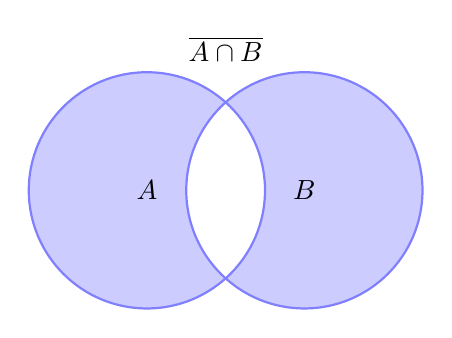
\begin{tikzpicture}
    [filled/.style={fill=blue!20, draw=blue!50, thick}, outline/.style={draw=blue!50, thick}]
    \draw[filled, even odd rule] (0,0) circle (1.5cm) node {$A$}
                                 (0:2cm) circle (1.5cm) node{$B$};
    \node[anchor=south] at (current bounding box.north) {$\overline{A \cap B}$};
\end{tikzpicture}
\end{center}
{\small (latex source from
\url{https://texample.net/tikz/examples/set-operations-illustrated-with-venn-diagrams/})}

\item Formally
  \begin{equation*}
    L(C)
=(L(A)\cap \overline{L(B)})\cup
(\overline{L(A)}\cap L(B))
  \end{equation*}
\item 
$B$ DFA $\Rightarrow$ so is $\overline{B}$

\item $A, B$ DFA $\Rightarrow$ so is 
$A\cup B, A\cap B$

\item Use $E_{DFA}$
\end{itemize}\end{frame} \begin{frame}[allowframebreaks] \frametitle{Decidability and CFL}
  \begin{itemize}
\item CFG
  \begin{equation*}
    A_{CFG}
=\{\langle  G,w\rangle \mid
G: CFG,\mbox{ generates } w\}
  \end{equation*}
\item We prove that $A_{CFG}$ is decidable
\item But an issue is the $\infty$ possible derivations of a CFG

\item For example,
  \begin{equation*}
  A\rightarrow B, B \rightarrow A
\end{equation*}

\item Chomsky normal form
  \begin{eqnarray*}
    && A \rightarrow BC\\
&& A \rightarrow a
  \end{eqnarray*}

\item Any $w, |w|=n$, derivation in 
exactly $2n-1$ steps

\item If $q$:\# rules, check $q^{2n-1}$ branches

\item Proof
  \begin{enumerate}
  \item Convert $G$ to Chomsky
  \item Check all $q^{2n-1}$ branches
  \end{enumerate}

  \item Results apply to PDA as well

\end{itemize}\end{frame} \begin{frame}[allowframebreaks] \frametitle{$E_{CFG}$}
\begin{equation*}
  E_{CFG}
=\{\langle  G\rangle \mid
G: CFG, L(G)=\emptyset\}
\end{equation*}
  \begin{itemize}
  \item idea: bottom up setting to see if any string can be generated
    from the start variable. From
  \begin{equation*}
    A\rightarrow a
  \end{equation*}
  We search if $\exists$
\begin{equation*}
  B\rightarrow A
\end{equation*}

\item Proof:
  \begin{enumerate}
  \item Mark all terminals
  \item Repeat until no new variables marked

  \item [] \quad if
    \begin{equation*}
    A\rightarrow U_1\cdots U_k
  \end{equation*}
   \quad and 
   \begin{equation*}
\text{all }    U_1, \ldots, U_k \text{ marked}
 \end{equation*}
\quad $\Rightarrow$  mark $A$
\item If start state marked, accept
\item [] Otherwise, reject
  \end{enumerate}
\end{itemize}\end{frame} \begin{frame}[allowframebreaks] \frametitle{$EQ_{CFG}$}
\begin{equation*}
  EQ_{CFG}
=\{\langle  G,H\rangle \mid G,H: CFG, L(G)=
L(H)\}
\end{equation*}
  \begin{itemize}
\item Remember that $EQ_{DFA}$ is decidable
\item However, we cannot apply the same proof as
 CFL is not closed for 
$\cap$ and complementation
\item It's proved in Chapter 5 that this language is not decidable
\item We do not discuss details
\end{itemize}\end{frame}

\begin{frame}[allowframebreaks] \frametitle{CFL decidable}
  \begin{itemize}
\item This question different from $A_{CFG}$ decidable
or not
\item How about converting PDA to a TM?
\item For nondeterministic PDA we can do NTM 
\item But nondeterministic PDA may have $\infty$-long branches

\item [] TM runs forever
\item So converting PDA to TM does not really work
\item A proof that works:

\item [] Find grammar $G$ for this CFL
\item [] Run TM for $\langle  G,w\rangle $ by using 
$A_{CFG}$
\end{itemize}\end{frame} \begin{frame}[allowframebreaks] \frametitle{Classes of languages}
  \begin{itemize}
  \item Fig 4.10

\begin{center}
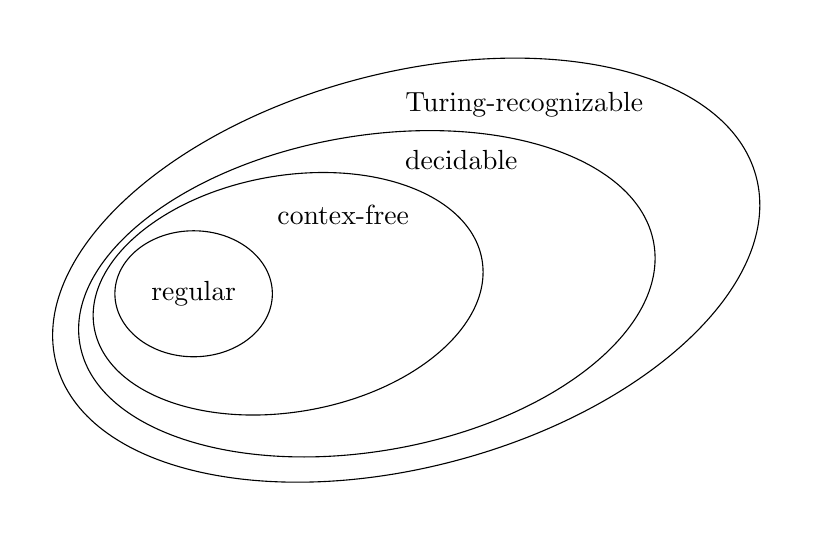
\begin{tikzpicture}
  % \draw (1,0) circle [radius=1.5];
  \draw (-3,0.3) circle [x radius=4.6cm, y radius=2.5cm, rotate=15];
  \draw (-3.5,0) circle [x radius=3.7cm, y radius=2cm, rotate=10];
  \draw (-4.5,0) circle [x radius=2.5cm, y radius=1.5cm, rotate=10];
  \draw (-5.7,0) circle [x radius=1cm, y radius=0.8cm];
  \path (-5.7,0) node {regular};
  \path (-3.8,1) node {contex-free};
  \path (-2.3,1.7) node {decidable};
  \path (-1.5,2.4) node {Turing-recognizable};  
\end{tikzpicture}
    \end{center}
\end{itemize}\end{frame} \begin{frame}[allowframebreaks] \frametitle{Halting problem}
  \begin{itemize}
\item We will show that this problem is not decidable
\item There quite a few undecidable problems:

\item [] For example, program verification are in general not solvable
\end{itemize}\end{frame} \begin{frame}[allowframebreaks] \frametitle{$A_{TM}$}
\begin{equation*}
  A_{TM}=\{
\langle  M,w\rangle \mid M: \mbox{ a TM that accepts } w\}
\end{equation*}
  \begin{itemize}
\item We will prove that $A_{TM}$ is undecidable
\item However, $A_{TM}$ is Turing recognizable

\item We can simply simulate $\langle  M,w\rangle $
\item To be decidable we hope to avoid an infinite loop

\item [] if at one point, know it cannot halt

$\Rightarrow$ reject
\item Thus this problem is called the halting problem
\end{itemize}\end{frame} \begin{frame}[allowframebreaks] \frametitle{Diagonalization method}
  \begin{itemize}
\item We need a technique called ``diagonalization method'' for the proof
\item It was developed by Cantor  in 1873
to check if two  infinite sets are equal

\item Example: consider
  \begin{center}
  set of even integers
\end{center}
versus
\begin{center}
set of $\{0,1\}^*$
\end{center}
\item Which one is larger ?
\item Definition: two sets are equal if elements
can be paired
\end{itemize}\end{frame} \begin{frame}[allowframebreaks] \frametitle{Definition 4.12}
  \begin{itemize}
\item $f$ is a one-to-one function if:
  \begin{equation*}
f(a)\neq f(b) \text{ if } a \neq b
\end{equation*}

\begin{center}
  \begin{tabular}{cc}
\begin{tikzpicture}
  \draw[->] (-1.5, 0) -- (1.5, 0) node[right] {$x$};
  \draw[->] (0, -0.5) -- (0, 2.2) node[above] {$y$};
  \draw[scale=0.5, domain=-2:2, smooth, variable=\x, blue] plot ({\x}, {\x*\x});
\end{tikzpicture}
    &
\begin{tikzpicture}
  \draw[->] (-0.5, 0) -- (2.2, 0) node[right] {$x$};
  \draw[->] (0, -1.3) -- (0, 1.5) node[above] {$y$};
  \draw[scale=0.5, domain=-2:2, smooth, variable=\y, red]  plot ({\y*\y}, {\y});
\end{tikzpicture}
  \end{tabular}
\end{center}
\item Left: a one-to-one function; right: not
\item $f:A\rightarrow B$ onto if 
  \begin{equation*}
\forall b \in B, \exists a \text{ such that } f(a)=b
\end{equation*}
\item Example:
  \begin{equation*}
    f(a) = a^2, \text{ where } A = (-\infty, \infty) \text{ and }
    B = (-\infty, \infty)
  \end{equation*}
  This is not an onto function because for $b = -1$, there is no
  $a$ such that $f(a) = b$
\item However, if we change it to
    \begin{equation*}
    f(a) = a^2, \text{ where } A = (-\infty, \infty) \text{ and }
    B = [0, \infty)
  \end{equation*}
it becomes an onto function
\item Definition: a function is called a
  correspondence if it is one-to-one and onto
\item Example:
      \begin{equation*}
    f(a) = a^3, \text{ where } A = (-\infty, \infty) \text{ and }
    B = (-\infty, \infty)
  \end{equation*}
\end{itemize}\end{frame} \begin{frame}[allowframebreaks] \frametitle{Example 4.13}
  \begin{itemize}
\item $N=\{1,2,\ldots\}$
\item $E=\{2,4,\ldots\}$
\item The two sets can be paired
  \begin{center}
    \begin{tabular}{cc}
$n$ & $f(n)=2n$\\ \hline
1 & 2 \\
2 & 4 \\
$\vdots$ & $\vdots$
    \end{tabular}
  \end{center}
\item We consider $N$ and $E$ have \alert{the same size}
\item Definition: a set is countable if it is 
  \begin{center}
finite or same size as $N$
\end{center}
\end{itemize}\end{frame} \begin{frame}[allowframebreaks] \frametitle{Rational Numbers Countable}
  \begin{itemize}
\item $Q=\{m/n
\mid m,n \in N\}$ countable


  \begin{center}
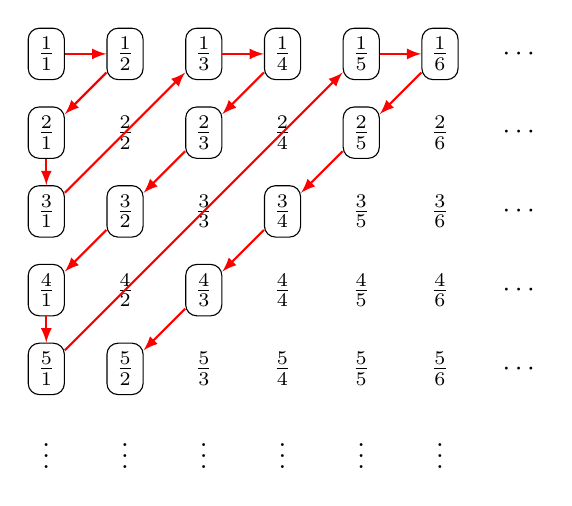
\begin{tikzpicture}
\tikzstyle{keepstyle} =[rectangle, rounded corners, draw, fill=white]
\node at (0,0) {$\vdots$};
\node[keepstyle] (51) at (0,1) {$\frac{5}{1}$};
\node[keepstyle] (41) at (0,2) {$\frac{4}{1}$};
\node[keepstyle] (31) at (0,3) {$\frac{3}{1}$};
\node[keepstyle] (21) at (0,4) {$\frac{2}{1}$};
\node[keepstyle] (11) at (0,5) {$\frac{1}{1}$};
\node at (1,0) {$\vdots$};
\node[keepstyle] (52) at (1,1) {$\frac{5}{2}$};
\node at (1,2) {$\frac{4}{2}$};
\node[keepstyle] (32) at (1,3) {$\frac{3}{2}$};
\node at (1,4) {$\frac{2}{2}$};
\node[keepstyle] (12) at (1,5) {$\frac{1}{2}$};
\node at (2,0) {$\vdots$};
\node at (2,1) {$\frac{5}{3}$};
\node[keepstyle] (43) at (2,2) {$\frac{4}{3}$};
\node at (2,3) {$\frac{3}{3}$};
\node[keepstyle] (23) at (2,4) {$\frac{2}{3}$};
\node[keepstyle] (13) at (2,5) {$\frac{1}{3}$};
\node at (3,0) {$\vdots$};
\node at (3,1) {$\frac{5}{4}$};
\node at (3,2) {$\frac{4}{4}$};
\node[keepstyle] (34) at (3,3) {$\frac{3}{4}$};
\node at (3,4) {$\frac{2}{4}$};
\node[keepstyle] (14) at (3,5) {$\frac{1}{4}$};
\node at (4,0) {$\vdots$};
\node  at (4,1) {$\frac{5}{5}$};
\node at (4,2) {$\frac{4}{5}$};
\node at (4,3) {$\frac{3}{5}$};
\node[keepstyle] (25) at (4,4) {$\frac{2}{5}$};
\node[keepstyle] (15) at (4,5) {$\frac{1}{5}$};
\node at (5,0) {$\vdots$};
\node  at (5,1) {$\frac{5}{6}$};
\node at (5,2) {$\frac{4}{6}$};
\node at (5,3) {$\frac{3}{6}$};
\node at (5,4) {$\frac{2}{6}$};
\node[keepstyle] (16) at (5,5) {$\frac{1}{6}$};
\node at (6,1) {$\cdots$};
\node at (6,2) {$\cdots$};
\node at (6,3) {$\cdots$};
\node at (6,4) {$\cdots$};
\node at (6,5) {$\cdots$};
\draw [-latex,red, thick] (11) -- (12);
\draw [-latex, red, thick] (12) -- (21);
\draw [-latex, red, thick] (21) -- (31);
\draw [-latex, red, thick] (31) -- (13);
\draw [-latex, red, thick] (13) -- (14);
\draw [-latex, red, thick] (14) -- (23);
\draw [-latex, red, thick] (23) -- (32);
\draw [-latex, red, thick] (32) -- (41);
\draw [-latex, red, thick] (41) -- (51);
\draw [-latex, red, thick] (51) -- (15);
\draw [-latex, red, thick] (15) -- (16);
\draw [-latex, red, thick] (16) -- (25);
\draw [-latex, red, thick] (25) -- (34);
\draw [-latex, red, thick] (34) -- (43);
\draw [-latex, red, thick] (43) -- (52);
\end{tikzpicture}
\end{center}

{\small Latex source from \url{https://divisbyzero.com/2013/04/16/countability-of-the-rationals-drawn-using-tikz/})}

\item Note that we skip counting elements with common factors (e.g., $2/2$)
\end{itemize}\end{frame} \begin{frame}[allowframebreaks] \frametitle{Real Numbers not Countable}
  \begin{itemize}
\item by diagonalization method
\item By contradiction
\item 

  \begin{tabular}{r|r}
$n$ & $f(n)$ \\ \hline
1 & 3.14159 $\ldots$\\
2 & 55.55555$\ldots$\\
3 & 0.12345 $\ldots$ \\
4 & 0.50000 $\ldots$ \\
$\vdots$ & 
  \end{tabular}

\item $x=0.4641\ldots$

$4\neq 1, 6 \neq 5$
\item $x \neq f(n), \forall n$
\item avoid problem $1=0.9999\cdots$

never choose 0 or 9
\end{itemize}\end{frame} \begin{frame}[allowframebreaks] \frametitle{Some languages not Turing-recognizable}
    \begin{itemize}
\item $\Sigma^*$ countable

count $|w|=1,2,3,\ldots$
\item sets of TM countable

$M$ can be represented as a finite string 

thinking about binary representation

subset of $\{0,1\}^*$


\item $L$: all languages over $\Sigma$

$B$: all infinite binary sequences
\item $A\in L$

$A: 0 \{0,1\}^*$

$\Sigma^*=\{\epsilon,0,1,00,01,10,11,000,001,\ldots\}$

$A=\{0, 00, 01, 000, 001, \ldots\}$

$\chi_A= 0 1 0 11 00 11 \ldots$
\item One-to-one correspondence between $B$ and $L$

$B$ uncountable (like real numbers)

$L$ uncountable
\item Each TM $\Rightarrow$ handle one language in $L$

TM countable, $L$ not

some cannot be handled by TM
\end{itemize}\end{frame} \begin{frame}[allowframebreaks] \frametitle{Halting problem undecidable}
  \begin{itemize}
\item 
$A_{TM}
=\{(M,w)\mid M: \mbox{TM, accepts } w\}$

by contradiction
\item $H$: decider for $A_{TM}$

  \begin{equation*}
    H(\langle  M,w\rangle )=
    \begin{cases}
      \mbox{accept} & \mbox{ if } M \mbox{ accepts } w\\
\mbox{reject} & \mbox{ not}
    \end{cases}
  \end{equation*}
\item A new TM $D$ with $H$ as a subroutine

$D$: input $\langle  M\rangle $, $M$: a TM

run $H$ on $\langle  M,\langle  M\rangle \rangle $

output opposite of $H$

\item $M$ can be input of $M$

A C compiler can be written in C

Do not worry how this compiler is compiled


\item 
  \begin{equation*}
    D(\langle  M\rangle )
=
\begin{cases}
  \mbox{accept } & 
\mbox{ if } M \mbox{ rejects } \langle  M\rangle \\
\mbox{reject} & \mbox{accept}
\end{cases}
  \end{equation*}

\item 
  \begin{equation*}
    D(\langle  D\rangle )
=
\begin{cases}
  \mbox{accept } & 
\mbox{ if } D \mbox{ rejects } \langle  D\rangle \\
\mbox{reject} & \mbox{accept}
\end{cases}
  \end{equation*}

\item contradiction

\end{itemize}\end{frame} \begin{frame}[allowframebreaks] \frametitle{Diagonalization in the proof}
  \begin{itemize}
\item List of TM
  \begin{center}
    \begin{tabular}{c|ccc}
& $\langle  M_1\rangle $ & $\langle  M_2\rangle $ & $\langle  M_3\rangle $\\ \hline
$M_1$ & A & &A\\
$M_2$ & A & A &A\\
$\vdots$ &&&
    \end{tabular}
  \end{center}
blank: unknown if $M_1$ reject or loop

\item But $H$ knows the solution
  \begin{center}
    \begin{tabular}{c|cc}
& $\langle  M_1\rangle $ & $\langle  M_2\rangle $ \\ \hline
$M_1$ & A & R\\
$M_2$ & A & A \\
$\vdots$ &&
    \end{tabular}
  \end{center}

\item $D$ opposite of diag
  \begin{center}
    \begin{tabular}{c|cccc}
& $\langle  M_1\rangle $ & $\langle  M_2\rangle $ & $\ldots$ & $\langle  D\rangle $\\ \hline
$M_1$ & R & &&\\
$M_2$ &  & R && \\
&& & $\ddots$ & \\
$D$ &&&& ?
    \end{tabular}
  \end{center}

\end{itemize}\end{frame} \begin{frame}[allowframebreaks] \frametitle{co-Turing-recognizable Language}
  \begin{itemize}
\item A language: co-Turing-recognizable

if its complement Turing-recognizable
\item Decidable $\Leftrightarrow$
Turing-recognizable and co-Turing-recognizable
\item $A_{TM}$ Turing-recognizable but not decidable

$\overline{A_{TM}}$ not Turing-recognizable

\end{itemize}\end{frame} \begin{frame}[allowframebreaks] \frametitle{Theorem 4.22}
  \begin{itemize}
\item ``$\Rightarrow$''

Decidable $\Rightarrow$ Turing-recognizable

Complement $\Rightarrow$ decidable $\Rightarrow$
Turing-recognizable


\item why not: Turing-recognizable

$\Rightarrow$ complement Turing-recognizable

what if we swap $q_{accept},q_{reject}$ ?

\item $a \notin A$, loop

$a \in \overline{A}$, still loop

remember $\overline{A}$: Turing-recognizable means

given $a \in \overline{A}$, accept in a finite \#
steps.

\item ``$\Leftarrow$'' $A,\overline{A}$ Turing-recognizable,
Machines $M_1, M_2$
\item A new machine $M$

input $w$
\begin{enumerate}
\item Run $M_1,M_2$ in parallel
\item $M_1$ accept $\Rightarrow$ accept, 
$M_2$ accept $\Rightarrow$ reject
\end{enumerate}
\item Never infinity loop

$M$ accepts all strings in $A$, reject all not in $A$

$M$: a decider of $A$

\end{itemize}\end{frame}
\end{document}

%%% Local Variables:
%%% mode: latex
%%% TeX-master: t
%%% End:
